%!TEX root = main.tex
\begin{figure*}[!htb]
\begin{subfigure}[b]{0.9\textwidth}
\centering
\includegraphics[width=0.9\textwidth]{latency_analysis}
\caption{
%\iap\ Cluster Emergency Response Latency : Shown is the 
This is the time between reception of the \emph{scatter} command by satellite 1 and the activation of the thrusters on each satellite, corresponding to interactions \textit{CommandProxy} to \textit{ModuleProxy}. The three regions of the plot indicate the three scenarios: (1) image processing application has limited use of its partitions and has a hyperperiod of 250 $ms$, (2) image processing application has full use of its partitions and has a hyperperiod of 250 $ms$, and (3) image processing application has full use of its partitions and has a hyperperiod of 100 $ms$.  The averages and variances for the satellites' latencies are shown for each of the three scenarios.}
\label{fig:latency_analysis}
\end{subfigure}
\begin{subfigure}[b]{0.9\textwidth}
\centering
\includegraphics[width=0.9\textwidth]{mixed_criticality_plot}
\caption{The engine activation following reception of a \emph{scatter} command is annotated for the relevant actors for scenario 2 shown above. The \emph{scatter} command causes the \emph{TrajectoryPlanning} to request \emph{ModuleProxy} to activate the thrusters for 500 $ms$. Notice that the image processing does not run while the mission-critical tasks are executing - without halting the partition scheduling.  Also note that the context switching during the execution of the critical tasks is the execution of the secure transport kernel thread. Only the application tasks are shown in the log; the kernel threads and other background processes are left out for clarity.}
\label{fig:orbiter_plot}
\end{subfigure}
\vspace{-0.1in}
%\vspace{-0.1in}
\caption{\iap\ Mixed Criticality Demo }
\vspace{-0.2in}
\end{figure*}

\section{Experiment: A 3-node Satellite Cluster}
\label{sec:experiment}

To demonstrate the DREMS platform, a multi-computing node experiment was created on a cluster of fanless computing nodes with a 1.6 GHz Intel Atom N270 processor and 1 GB of RAM each. 
On these nodes, a cluster of three satellites was emulated and each satellite ran the example applications described in Section~\ref{sec:intro}. 
% We use these example applications to show that the performance of mission-critical tasks is not affected by application tasks. 
  Because the performance of the cluster flight control application is of interest, we explain the interactions between its actors below.  

\begin{figure}[t]
\centering
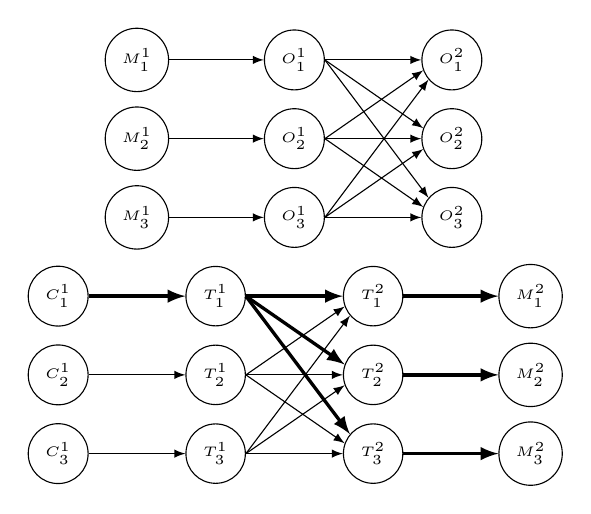
\begin{tikzpicture}[x=1cm,y=1cm, 
taskW/.style={shape=circle,draw,align=center,font=\tiny,text=white},
taskB/.style={shape=circle,draw,align=center,font=\tiny}]
%% define origos: uxo = upper x origo; uyo = upper y origo; lxo = lower x origo; lyo = lower y origo
\def\uxo{0}\def\uyo{3}\def\lxo{0}\def\lyo{0}
\node[taskB](M11) at (\uxo-2,\uyo+1) {$M^1_1$}; \node[taskB](V11) at (\uxo,\uyo+1) {$O^1_1$}; \node[taskB](V21) at (\uxo+2,\uyo+1) {$O^2_1$};
\node[taskB](M12) at (\uxo-2,\uyo) {$M^1_2$};   \node[taskB](V12) at (\uxo,\uyo) {$O^1_2$};   \node[taskB](V22) at (\uxo+2,\uyo) {$O^2_2$};
\node[taskB](M13) at (\uxo-2,\uyo-1) {$M^1_3$}; \node[taskB](V13) at (\uxo,\uyo-1) {$O^1_3$}; \node[taskB](V23) at (\uxo+2,\uyo-1) {$O^2_3$};
\draw[-latex] (M11.0) -- (V11.180); \draw[-latex] (M12.0) -- (V12.180); \draw[-latex] (M13.0) -- (V13.180);
\draw[-latex] (V11.0) -- (V21.180); \draw[-latex] (V12.0) -- (V21.200); \draw[-latex] (V13.0) -- (V21.220);
\draw[-latex] (V11.0) -- (V22.160); \draw[-latex] (V12.0) -- (V22.180); \draw[-latex] (V13.0) -- (V22.200);
\draw[-latex] (V11.0) -- (V23.140); \draw[-latex] (V12.0) -- (V23.160); \draw[-latex] (V13.0) -- (V23.180);
%%%
\node[taskB](C11) at (\lxo-3,\lyo+1) {$C^1_1$}; \node[taskB](O11) at (\lxo-1,\lyo+1) {$T^1_1$}; \node[taskB](O21) at (\lxo+1,\lyo+1) {$T^2_1$}; \node[taskB](M21) at (\lxo+3,\lyo+1) {$M^2_1$};
\node[taskB](C12) at (\lxo-3,\lyo)   {$C^1_2$}; \node[taskB](O12) at (\lxo-1,\lyo)   {$T^1_2$}; \node[taskB](O22) at (\lxo+1,\lyo)   {$T^2_2$}; \node[taskB](M22) at (\lxo+3,\lyo) {$M^2_2$};
\node[taskB](C13) at (\lxo-3,\lyo-1) {$C^1_3$}; \node[taskB](O13) at (\lxo-1,\lyo-1) {$T^1_3$}; \node[taskB](O23) at (\lxo+1,\lyo-1) {$T^2_3$}; \node[taskB](M23) at (\lxo+3,\lyo-1) {$M^2_3$};
\draw[-latex,very thick] (C11.0) -- (O11.180); \draw[-latex] (C12.0) -- (O12.180); \draw[-latex] (C13.0) -- (O13.180);
\draw[-latex,very thick] (O11.0) -- (O21.180); \draw[-latex] (O12.0) -- (O21.200); \draw[-latex] (O13.0) -- (O21.220);
\draw[-latex,very thick] (O11.0) -- (O22.160); \draw[-latex] (O12.0) -- (O22.180); \draw[-latex] (O13.0) -- (O22.200);
\draw[-latex,very thick] (O11.0) -- (O23.140); \draw[-latex] (O12.0) -- (O23.160); \draw[-latex] (O13.0) -- (O23.180);
\draw[-latex,very thick] (O21.0) -- (M21.180); \draw[-latex,very thick] (O22.0) -- (M22.180); \draw[-latex,very thick] (O23.0) -- (M23.180);
\end{tikzpicture}%
\vspace{1.5mm}

\begin{footnotesize}
\begin{tabular}{| c | c | c | p{4cm} |}
\hline
Task & Actor & Activity \\ [0.5ex]
\hline
$M^1$ & \multirow{2}{*}{$ModuleProxy$} &  Inform $O^1$ of new state\\
\cline{1-1}\cline{3-3}
$M^2$ & & Activate engine\\
\hline
$O^1$ & \multirow{2}{*}{$OrbitalMaintenance$} & Publish new state\\
\cline{1-1}\cline{3-3}
$O^2$ & & Subscribe to new state\\
\hline
$T^1$ & \multirow{2}{*}{$TrajectoryPlanning$} & Publish new command\\
\cline{1-1}\cline{3-3}
$T^2$ & & Subscribe to new command\\
\hline
$C^1$ & $CommandProxy$ & Inform $T^1$ of command\\
\hline
\end{tabular}
\end{footnotesize}

\caption{\iap\ tasks : 
\emph{ModuleProxy} tasks control thruster activation in Orbiter and state vector retrieval from Orbiter.
\emph{OrbitalMantenance} tasks track the cluster satellites' state vectors and disseminate them.  
\emph{TrajectoryPlanning} tasks control the response to commands and satellite thruster activation.
\emph{CommandProxy} tasks inform the satellite of a command from the ground network.  
For these tasks, the subscript represents the node ID on which the task is deployed.
The total latency of the interaction $C_1^1 \to M_N^2$ represents the total emergency response latency
between receiving the \emph{scatter} command and activating the thrusters.  This interaction pathway 
is shown in bold.
}
\label{fig:OrbiterDemoTDG}
\vspace{-0.2in}
\end{figure}

The mission-critical cluster flight application (CFA) (Figure \ref{fig:OrbiterDemoTDG}) consists of four actors: \emph{OrbitalMaintenance}, \emph{TrajectoryPlanning}, \emph{CommandProxy}, and \emph{ModuleProxy}. \emph{ModuleProxy} connects to the Orbiter space
flight simulator (\url{http://orbit.medphys.ucl.ac.uk/}) that simulates the satellite hardware and orbital mechanics for the three satellites in low Earth orbit. \emph{CommandProxy} receives commands from the ground network.  \emph{OrbitalMaintenance} keeps track of every satellite's position and updates the cluster with its current position. This is done by a group publish subcribe interaction between all \textit{OrbitalMaintenance} actors across all nodes.  
% These CFA tasks and their interactions are further explained in Figure~\ref{fig:OrbiterDemoTDG}. 

 Additionally, four image processing application (IPA) actors (one
 actor per application instance) are deployed as application
 tasks. The IPA design allows the percentage of CPU cycles consumed by
 them to be configurable.  The four IPAs are  
 assigned to two partitions, such that each partition contains two IPA
 actors.  A third, shorter, partition runs the
 \emph{OrbitalMaintenance} actor; since it is a periodic task, it
 updates the satellite state every second and is not critical in an
 emergency.   
% please describe the partition assignment.

% A sample scheduler log from node $1$ is shown in Figure~\ref{fig:orbiter_plot} and demonstrates the proper preemption of the image processing tasks by the critical CFA tasks.

\iffalse
To ensure the cluster safety, the latency between the reception of the command from the ground station and the activation of the satellites' thrusters should be minimized, \emph{i.e.} regardless of other applications, the latency of the interaction 
% $C_1^1 \to M_N^2$, described in Figure~\ref{fig:OrbiterDemoTDG}, 
between the \textit{CommandProxy} and the \textit{ModuleProxy}
should remain as small as possible.  Note: since only the cluster leader (node \emph{1}) receives the scatter command, \emph{CommandProxy} and command publish on nodes \emph{2} and \emph{3} are not active.   
These latencies were calculated from time-stamped messages; using NTP (\url{http://www.ntp.org}), all nodes' clocks were synchronized. % to within 10 $\mu s$. 
\fi
Figures~\ref{fig:latency_analysis} and~\ref{fig:orbiter_plot} show the results from three different scenarios: 1) hyperperiod of 250 ms, with IPA consuming less than 50 percent CPU. 2)  hyperperiod of 250 ms, with IPA consuming 100 percent CPU and 3)  hyperperiod of 100 ms, with IPA consuming 100 percent CPU. As shown in figure ~\ref{fig:latency_analysis}, the emergency response latency over the three nodes was quite low with very little variance, and did not correlate with either the image application's CPU utilization or the application's partition schedule.  Since we show that the emergency response has very low latency with little variance between different application loads on the system, we provide a stable platform for deterministic and reliable emergency response.  As such, the satellite cluster running the \iap\ infrastructure is able to quickly respond to emergency situations despite high application CPU load and without altering the partition scheduling.  Figure~\ref{fig:orbiter_plot}  demonstrates the proper preemption of the image processing tasks by the critical CFA tasks for scenario 2.
